\documentclass[9pt,twocolumn,twoside]{osajnl}
% \documentclass[11pt,twocolumn,twoside]{osajnl}
\usepackage{caption,graphicx,subcaption,overpic,tikz,tkz-tab,verbatim,multirow,booktabs,siunitx,amsmath,amssymb,bm,mathtools,threeparttable,color,enumitem,listingsutf8,url,xcolor,etaremune,bibentry,textcomp,mathpazo,geometry,lastpage,fancyhdr,float,epstopdf}

\journal{ol} % Choose journal (ao, aop, josaa, josab, ol, pr)

% See template introduction for guidance on setting shortarticle option
\setboolean{shortarticle}{true}
% true = letter / tutorial
% false = research / review article
% (depending on journal).

\title{Volumetric on-axis holographic imaging}

\author[ ]{Ni Chen}
\author[*]{Byoungho Lee}
% \author[1]{Author Three}

\affil[1]{Department of Electrical and Computer Engineering,
Seoul National University, Seoul 08826, Korea}
% \affil[2]{School of Science, University of Technology, 2000 J St. NW, Washington DC, 20036}
% \affil[3]{School of Optics, University of Technology, 2000 J St. NW, Washington DC, 20036}

\affil[*]{Corresponding author: byoungho@snu.ac.kr}

%% To be edited by editor
% \dates{Compiled \today}

%\ociscodes{(140.3490) Lasers, distributed feedback; (060.2420) Fibers, polarization-maintaining;(060.3735) Fiber Bragg gratings.}

%% To be edited by editor
% \doi{\url{http://dx.doi.org/10.1364/XX.XX.XXXXXX}}


\graphicspath{{./figure/}}

\begin{abstract}
This legacy template can be used to prepare a research article for submission to OSA’s journals \emph{Applied Optics}, \emph{Advances in Optics and Photonics}, JOSA A, JOSA B, and \emph{Optics Letters}. \emph{Optics Letters} authors may use this template for a precise length estimate. Use the shortarticle/true option for \emph{Optics Letters}. Please note that OSA is no longer using OCIS codes. 
\end{abstract}

\setboolean{displaycopyright}{true}

\begin{document}

\maketitle

\section{Introduction}

Gabor hologram:
\begin{equation}
I_{Gabor} = |o + r|^2 = |r|^2 + |o|^2 + o^*r + or^*
\label{eq_gabor}
\end{equation}
After normalization, $I_{Gabor} \approx o^*r + or^*$.

\section{Examples of Article Components}\label{sec:examples}

The sections below show examples of different article components.

\section{Figures and Tables}

It is not necessary to place figures and tables at the back of the manuscript. Figures and tables should be sized as they are to appear in the final article. Do not include a separate list of figure captions and table titles.

Figures and Tables should be labelled and referenced in the standard way using the \verb|\label{}| and \verb|\ref{}| commands.

\subsection{Sample Figure}

\begin{figure}[htbp]
\centering
\begin{subfigure}[b]{1\linewidth}
\centering
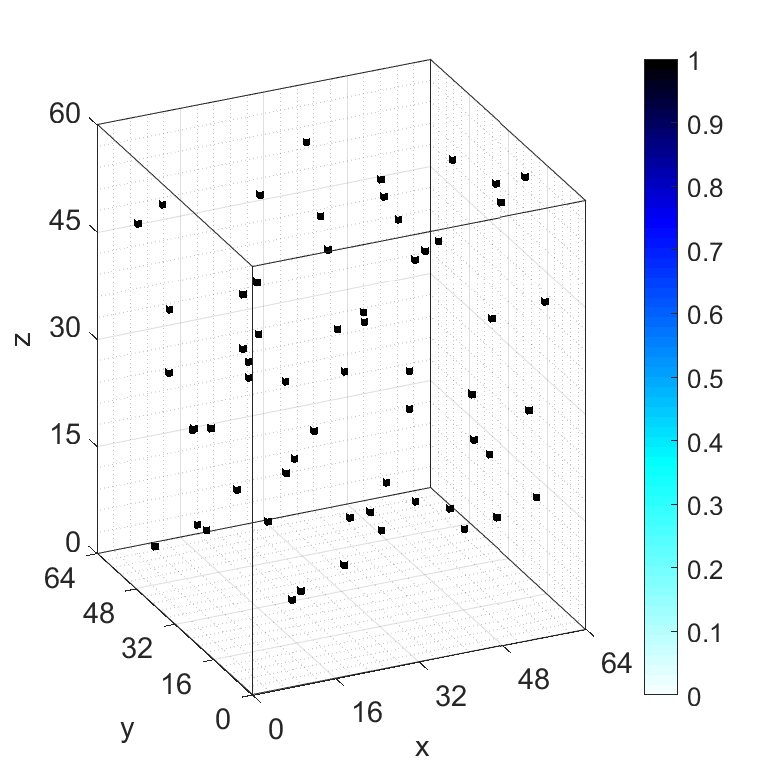
\includegraphics[width=0.3\linewidth]{random}
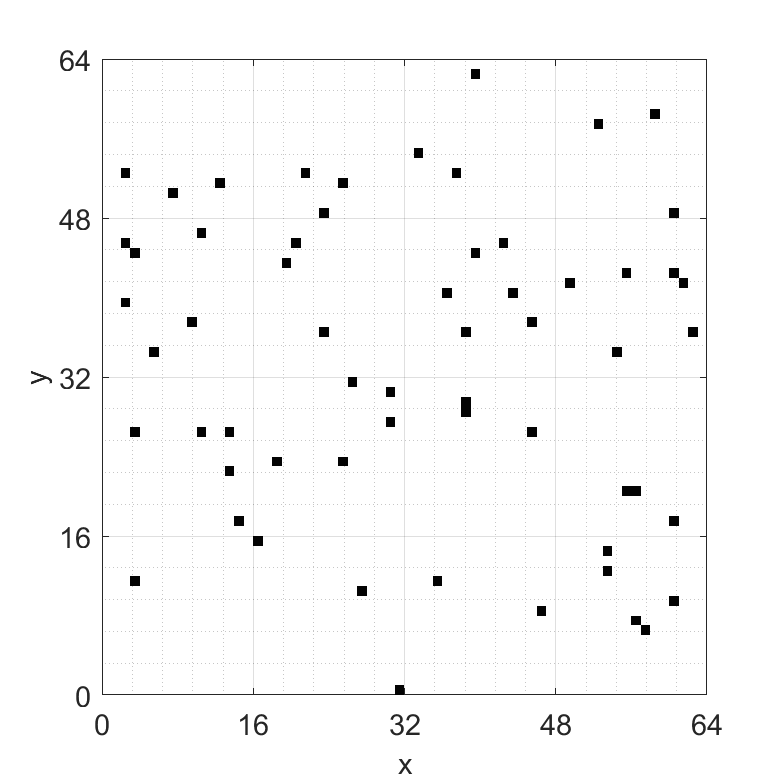
\includegraphics[width=0.3\linewidth]{random_top}
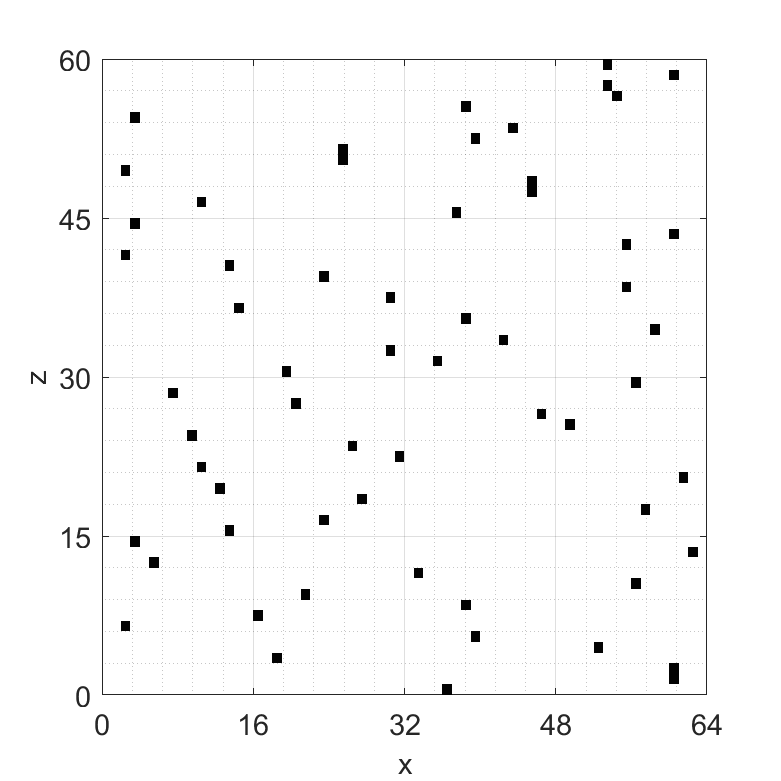
\includegraphics[width=0.3\linewidth]{random_side}
\caption{Original Object}
\end{subfigure}

\begin{subfigure}[b]{1\linewidth}
\centering
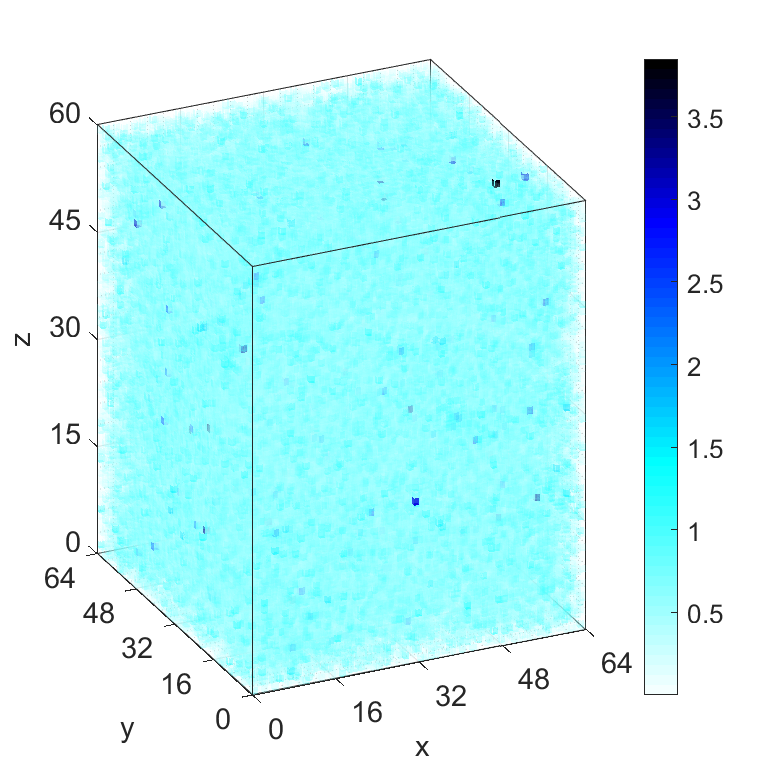
\includegraphics[width=0.3\linewidth]{random_inline_BP_3d}
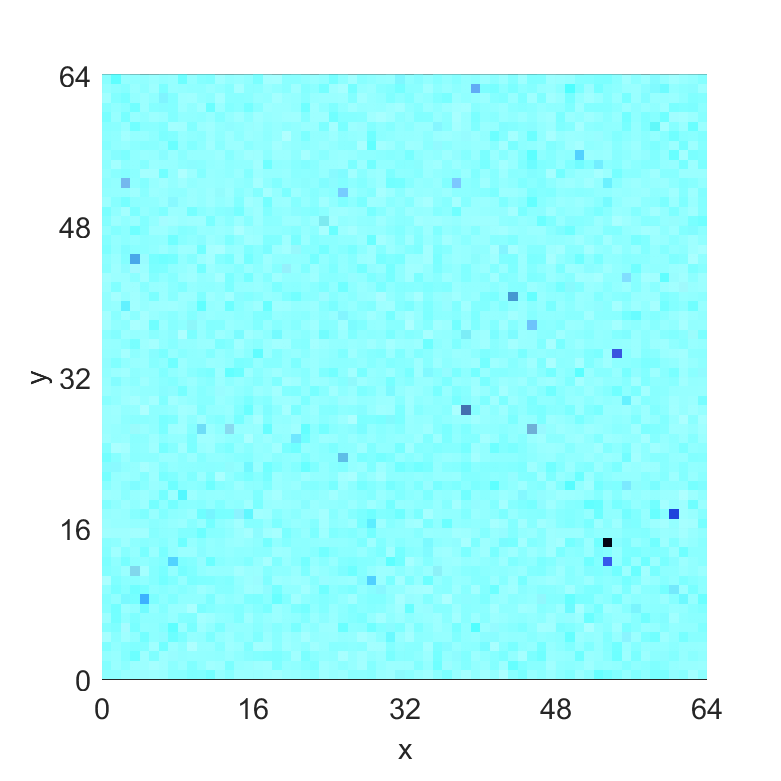
\includegraphics[width=0.3\linewidth]{random_inline_BP_top}
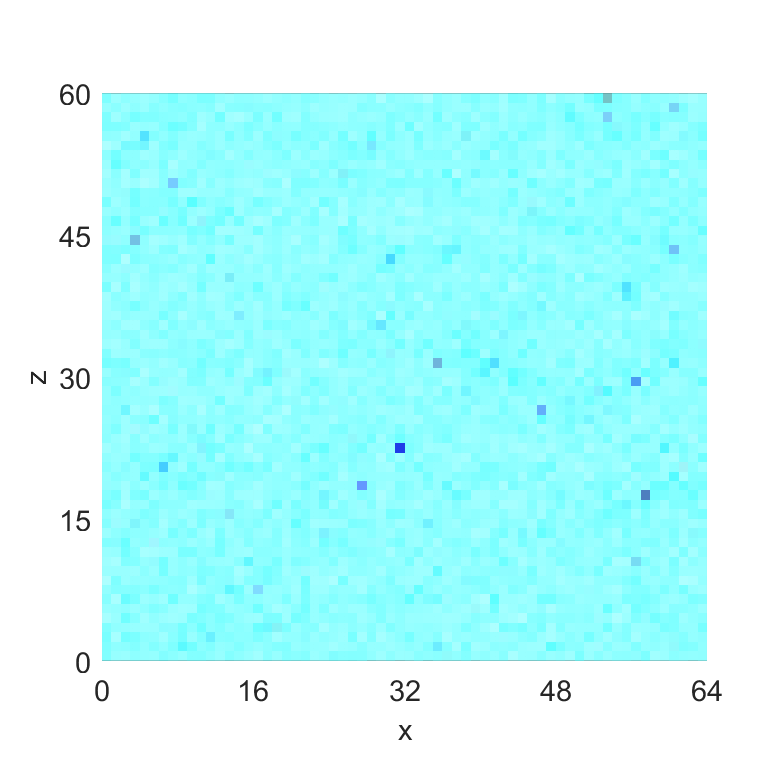
\includegraphics[width=0.3\linewidth]{random_inline_BP_side}
\caption{Back propagation}
\end{subfigure}

\begin{subfigure}[b]{1\linewidth}
\centering
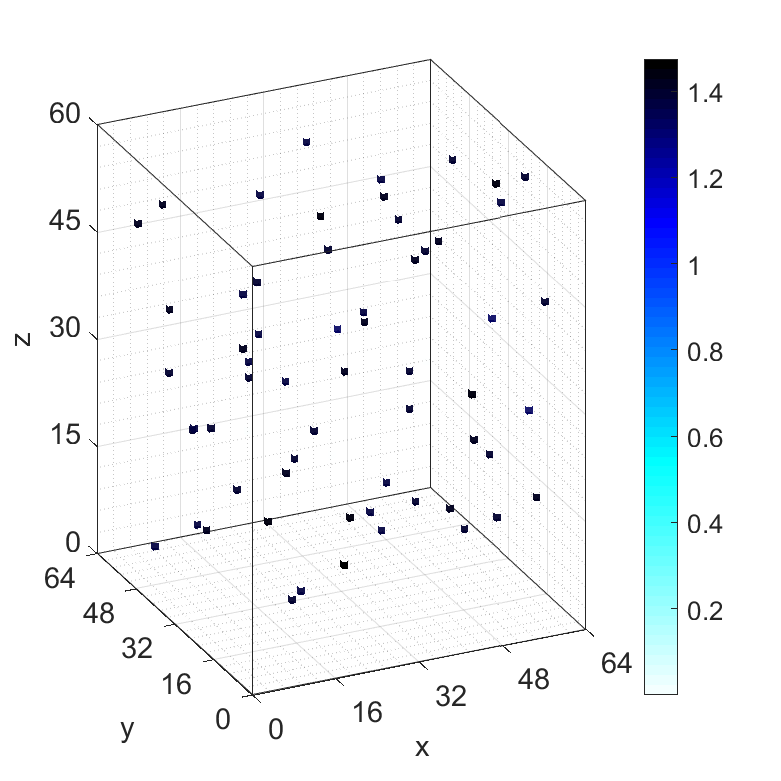
\includegraphics[width=0.3\linewidth]{random_inline_TwIST_3d}
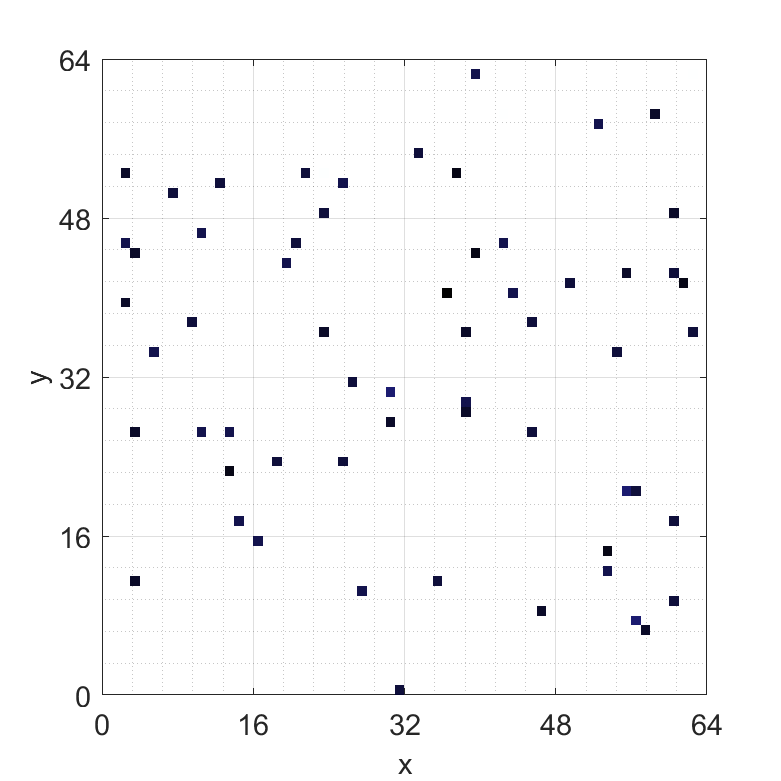
\includegraphics[width=0.3\linewidth]{random_inline_TwIST_top}
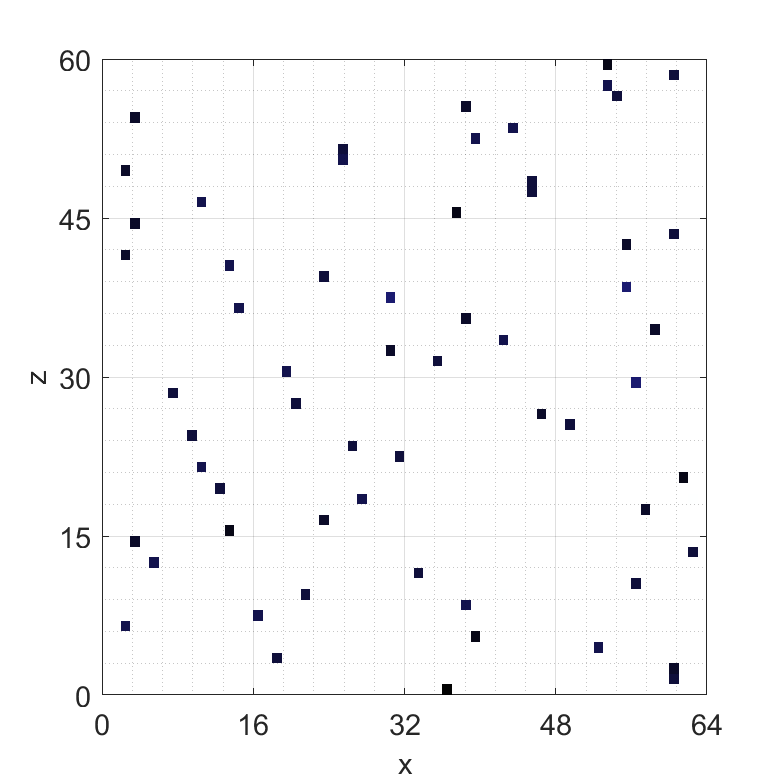
\includegraphics[width=0.3\linewidth]{random_inline_TwIST_side}
\caption{Complex Deconvolution}
\end{subfigure}

\caption{Simulation with a random scattering object (Gaussian noise with 35db)}
\label{fig_sim_random}
\end{figure}

\subsection{Sample Table}

Table \ref{tab:shape-functions} shows an example table.

\begin{table}[htbp]
\centering
\caption{\bf Shape Functions for Quadratic Line Elements}
\begin{tabular}{ccc}
\hline
local node & $\{N\}_m$ & $\{\Phi_i\}_m$ $(i=x,y,z)$ \\
\hline
$m = 1$ & $L_1(2L_1-1)$ & $\Phi_{i1}$ \\
$m = 2$ & $L_2(2L_2-1)$ & $\Phi_{i2}$ \\
$m = 3$ & $L_3=4L_1L_2$ & $\Phi_{i3}$ \\
\hline
\end{tabular}
  \label{tab:shape-functions}
\end{table}

\section{Sample Equation}

Let $X_1, X_2, \ldots, X_n$ be a sequence of independent and identically distributed random variables with $\text{E}[X_i] = \mu$ and $\text{Var}[X_i] = \sigma^2 < \infty$, and let
\begin{equation}
S_n = \frac{X_1 + X_2 + \cdots + X_n}{n}
      = \frac{1}{n}\sum_{i}^{n} X_i
\label{eq:refname1}
\end{equation}
denote their mean. Then as $n$ approaches infinity, the random variables $\sqrt{n}(S_n - \mu)$ converge in distribution to a normal $\mathcal{N}(0, \sigma^2)$.

\section{Sample Algorithm}

Algorithms can be included using the commands as shown in algorithm \ref{alg:euclid}.

\begin{algorithm}
\caption{Euclid’s algorithm}\label{alg:euclid}
\begin{algorithmic}[1]
\Procedure{Euclid}{$a,b$}\Comment{The g.c.d. of a and b}
\State $r\gets a\bmod b$
\While{$r\not=0$}\Comment{We have the answer if r is 0}
\State $a\gets b$
\State $b\gets r$
\State $r\gets a\bmod b$
\EndWhile\label{euclidendwhile}
\State \textbf{return} $b$\Comment{The gcd is b}
\EndProcedure
\end{algorithmic}
\end{algorithm}

\section{Supplemental Material}

Consult the Author Guidelines for Supplementary Materials in OSA Journals for details on accepted types of materials and instructions on how to cite them.
All materials must be associated with a figure, table, or equation or be referenced in the results section of the manuscript.
(1) 2D and 3D image files and video must be labeled “Visualization,” not “Movie,” “Video,” “Figure,” etc.
(2) Machine-readable data (for example, csv files) must be labeled  “Data File.”  Number data files and visualizations consecutively, e.g., “Visualization 1, Visualization 2….”
(3) Large datasets or code files must be placed in an open, archival database.  Such items should be mentioned in the text as either “Dataset” or “Code,” as appropriate, and also be cited in the references list.  For example, “see Dataset 1 (Ref. [1]) and Code 1 (Ref [2]).” Here are examples of the references:

\subsection{Sample Dataset Citation}

1. M. Partridge, "Spectra evolution during coating," figshare (2014) [retrieved 13 May 2015], http://dx.doi.org/10.6084/m9.figshare.1004612.

\subsection{Sample Code Citation}

2. C. Rivers, "Epipy: Python tools for epidemiology" (Figshare, 2014) [retrieved 13 May 2015], http://dx.doi.org/10.6084/m9.figshare.1005064.

\section{Funding Information}

Funding information should be listed in a separate block preceding any acknowledgments. List just the funding agencies and any associated grants or project numbers, as shown in the example below:

National Science Foundation (NSF) (1263236, 0968895, 1102301); The 863 Program (2013AA014402).

The acknowledgments may contain any information that is not related to funding:

The authors thank H. Haase, C. Wiede, and J. Gabler for technical support.

Do not use Funding Information or Acknowledgment headings.

\section{References}

Note that \emph{Optics Letters} uses an abbreviated reference style. Citations to journal articles should omit the article title and final page number; this abbreviated reference style is produced automatically when the \emph{Optics Letters} journal option is selected in the template, if you are using a .bib file for your references.

However, full references (to aid the editor and reviewers) must be included as well on a fifth informational page that will not count against page length; again this will be produced automatically if you are using a .bib file.

\bigskip
\noindent Add citations manually or use BibTeX. See \cite{Zhang:14,OSA,FORSTER2007,testthesis,manga_rao_single_2007}.

% Bibliography
\bibliography{3dholoref}

% Full bibliography added automatically for Optics Letters submissions; the following line will simply be ignored if submitting to other journals.
% Note that this extra page will not count against page length
\bibliographyfullrefs{3dholoref}



% Please include bios and photos of all authors for aop articles
\ifthenelse{\equal{\journalref}{aop}}{%
\section*{Author Biographies}
\begingroup
\setlength\intextsep{0pt}
\begin{minipage}[t][6.3cm][t]{1.0\textwidth} % Adjust height [6.3cm] as required for separation of bio photos.
  \begin{wrapfigure}{L}{0.25\textwidth}
    
\includegraphics[width=0.25\textwidth]{john_smith.eps}
  \end{wrapfigure}
  \noindent
  {\bfseries John Smith} received his BSc (Mathematics) in 2000 from The University of Maryland. His research interests include lasers and optics.
\end{minipage}
\begin{minipage}{1.0\textwidth}
  \begin{wrapfigure}{L}{0.25\textwidth}
    
\includegraphics[width=0.25\textwidth]{alice_smith.eps}
  \end{wrapfigure}
  \noindent
  {\bfseries Alice Smith} also received her BSc (Mathematics) in 2000 from The University of Maryland. Her research interests also include lasers and optics.
\end{minipage}
\endgroup
}{}


\end{document}
